% CISS 2027 practice submission (Johns Hopkins, Baltimore, 24--26 March 2027).
% Format per the CISS call (2023 call, the latest one readable; 2027 call not yet published):
% "Submissions in FINAL FORMAT and no longer than six (6) pages", IEEE conference format,
% IEEE Xplore proceedings. Not anonymous: the submission is the final manuscript.
% Condensed on 22 October 2026 from the KDD 2027 draft (kdd/submission/main.tex).
% Compile:  tectonic -X compile main.tex
\documentclass[conference]{IEEEtran}

% IEEEtran asks for Times (ptm), which XeTeX/tectonic lacks in TU encoding; load the Times clone.
\usepackage{iftex}
\ifXeTeX
  \usepackage{fontspec}
  \setmainfont{texgyretermes}[Extension=.otf, UprightFont=*-regular, BoldFont=*-bold,
    ItalicFont=*-italic, BoldItalicFont=*-bolditalic]
\fi

\usepackage{amsmath,amssymb,amsthm}
\usepackage{booktabs}
\usepackage{graphicx}
\usepackage{mathtools}
\usepackage{cite}
\usepackage[hidelinks]{hyperref}

\newtheorem{theorem}{Theorem}
\newtheorem{proposition}{Proposition}
\newcommand{\E}{\mathbb{E}}
\newcommand{\Var}{\mathrm{Var}}
\newcommand{\Cov}{\mathrm{Cov}}
\newcommand{\diag}{\operatorname{diag}}
\newcommand{\I}{\mathcal{I}}

\begin{document}

\title{When Can a Bandit Trust Correlation? Certified Pooling and Valid Confidence under Spatiotemporal Dependence}

% TODO before submission: CISS is not double-blind; fill in names and affiliations.
\author{\IEEEauthorblockN{Author Names}
\IEEEauthorblockA{Affiliation\\
City, State, USA\\
email@domain}}

\maketitle

\begin{abstract}
Recommendation platforms log graphs that suggest which items share appeal, and their rewards persist and move together for days. A bandit that pools along such a graph, or that treats feedback as independent, can fail. We model rewards as fixed long-run means plus autoregressive deviations with graph-correlated Gaussian innovations, and separate two roles of a graph: restricting the means or shaping the shocks. Only the first identifies unobserved arms. For the means, the regret of certified pooling depends on which components its certified widths make rejectable, and effective-resistance diameters miss the information geometry. For the shocks, an exact innovation regression turns adaptive, restless observations into a predictable Gaussian design, which gives confidence sets valid at all times and keeps certified pooling valid. Confidence built for independent rewards fails under bursty exposure by a computable autocorrelation inflation factor. On KuaiRec and the Open Bandit Dataset, certified gains track the share of rejectable components (Spearman $-0.87$ across certificates), while graph-free shrinkage matches graph-based pooling on average. Held-out Wikipedia attention shows the predicted inflation: a week of views carries the information of 1.3--1.9 independent days, and on worlds calibrated to it, independence-based certificates fail in 56--94\% of runs while innovation certificates show no failures but are too wide to eliminate arms.
\end{abstract}

\begin{IEEEkeywords}
multi-armed bandits, graph side information, autoregressive rewards, confidence sequences, Kalman filtering
\end{IEEEkeywords}

%=====================================================================
\section{Introduction}
%=====================================================================

A short-video platform fills a trending slot every day, and its rewards are correlated in two ways. \emph{Across arms}, videos close in a co-engagement graph tend to share long-run appeal, and a shock such as a holiday hits related videos together. \emph{Over time}, a video's engagement today predicts its engagement for days. Graph bandits assume the first as a static restriction on means~\cite{valko2014spectral,ban2021local}. Restless and autoregressive bandits assume the second, usually with independent arms~\cite{chen2023autoregressive,trella2025latent}. We study both together and ask two inference questions: which logged correlation can a learner trust, and when do its confidence statements break?

A learner can go wrong in two ways. It can trust spatial correlation that is not there: pooling along a graph whose neighbourhoods do not share appeal biases estimates and can cause linear regret. Or it can ignore temporal correlation: confidence sets built for independent rewards are too narrow when consecutive observations move together, so irrevocable decisions such as dropping an arm go wrong.

\paragraph*{Contributions}
\begin{enumerate}
\item A reward model in which a graph can restrict the long-run means or shape the innovation covariance, with a node--time covariance that is separable only under homogeneous dynamics (Section~\ref{sec:model}).
\item For the means, a regret bound for certified pooling that depends on which components are rejectable, and a path--clique separation showing that diameters miss information geometry (Section~\ref{sec:pool}).
\item For the shocks, an exact innovation regression that yields all-time confidence under adaptive restless sampling and keeps certified pooling valid, and the inflation factor by which independence-based confidence fails under bursts (Section~\ref{sec:info}).
\item Tests of each prediction on KuaiRec~\cite{gao2022kuairec}, the Open Bandit Dataset~\cite{saito2021obd} and Wikipedia attention (Section~\ref{sec:evidence}).
\end{enumerate}

%=====================================================================
\section{A spatiotemporal reward model}\label{sec:model}
%=====================================================================

There are $N$ arms. Arm $i$'s reward field is
\begin{equation}\label{eq:model}
\begin{gathered}
X_{i,t}=\mu_i+z_{i,t},\qquad z_{i,t}=\textstyle\sum_{r=1}^{p_i}a_{i,r}z_{i,t-r}+\eta_{i,t},\\
\eta_t\stackrel{\rm iid}{\sim}N(0,Q_G).
\end{gathered}
\end{equation}
In round $t$ the learner chooses $a_t$ and observes $Y_t=X_{a_t,t}+\xi_t$ with sensor noise $\xi_t\sim N(0,r)$. Every arm evolves every round (restless), but only chosen arms are observed. The means $\mu$ are fixed and unknown, $Q_G\succ0$, and the field starts in stationarity. The AR polynomials $A_i(s)=1-\sum_ra_{i,r}s^r$ are stable, with $c_i=A_i(1)$. For the theory the dynamics, $Q_G$ and $r$ are known; Section~\ref{sec:evidence} tests estimated dynamics.

\paragraph*{Two roles for a graph} A graph with Laplacian $L_\mu$ may restrict the \emph{means}: $\mu^\top L_\mu\mu\le S^2$ and $\|\mu\|\le B$. For vertices in one connected component, effective resistance then bounds differences, $|\mu_i-\mu_j|\le S\sqrt{(e_i-e_j)^\top L_\mu^\dagger(e_i-e_j)}$. A graph with Laplacian $L_\eta$ may instead shape the \emph{shocks}, for example $Q_G\propto(\alpha_\eta I+\lambda_\eta L_\eta)^{-1}$. The roles differ in identification: correlated shocks improve prediction and comparisons, but an arm that is never observed has a zero column in the design, so its mean does not enter the likelihood. Only a mean restriction links an unobserved arm to observed ones.

\paragraph*{Space meets time} Stack each arm's deviation and lags into $s_t$, so $s_{t+1}=Fs_t+E\eta_{t+1}$ and $z_t=Cs_t$ with $F$ block-diagonal (AR companion blocks), $E$ inserting innovations, and $C=E^\top$. The stationary covariance solves $\Gamma=F\Gamma F^\top+EQ_GE^\top$; although $F$ is block-diagonal, $EQ_GE^\top$ couples the arms.

\begin{proposition}[Node--time covariance]\label{prop:cov}
Let $G_h=\Cov(z_{t+h},z_t)$ and let $\psi_i$ be arm $i$'s impulse response. Then $(G_h)_{ij}=(Q_G)_{ij}\sum_{k\ge0}\psi_i(k+h)\psi_j(k)$, and the spectral density is $\mathcal S_z(\omega)=\Lambda(\omega)Q_G\Lambda(\omega)^*$ with $\Lambda(\omega)=\diag(A_i(e^{-{\rm i}\omega})^{-1})$. The covariance is a fixed spatial matrix times a scalar temporal kernel if and only if all arms share one impulse response; otherwise $G_h$ is generally asymmetric for $h>0$.
\end{proposition}

\begin{IEEEproof}[Sketch]
Innovations at different dates are independent, so only equal-date terms of the causal expansions survive. For the converse, separability forces equal normalized autocorrelations, and a stable causal AR transfer is the unique minimum-phase factor of its spectrum.
\end{IEEEproof}

Consequently an AR(20) arm can have no lag-1 correlation but strong lag-20 correlation, and a lag-one persistence summary misstates how much a schedule reveals.

\paragraph*{Regret} \emph{Mean regret} $R_\mu(T)=\sum_t(\mu^\star-\mu_{a_t})$ measures learning of persistent appeal; \emph{dynamic regret} $\sum_t(\max_iX_{i,t}-X_{a_t,t})$ measures tracking of the current field. iid bandits ($p_i=0$, diagonal $Q_G$), graph bandits (mean restriction only) and restless AR bandits (no mean restriction) are special cases.

%=====================================================================
\section{Trusting a graph for the means}\label{sec:pool}
%=====================================================================

Assume first iid centered $\sigma^2$-sub-Gaussian noise. SP-UCB partitions the arms into $M$ components $C_c$ with supplied widths $\varepsilon_c\ge\max_{i,j\in C_c}|\mu_i-\mu_j|$. With $b(n)=\sqrt{2\sigma^2\ell/n}$ and $\ell=\log(2(N+M)T/\delta)$, it forms arm bounds $\bar Y_i+b(n_i)$ and pooled bounds $\hat p_c+b(N_c)+\varepsilon_c$, selects the component maximizing the smaller of its two bounds, and pulls that component's best arm. Let $v_c=\max_{i\in C_c}\mu_i$, $\Gamma_c=\mu^\star-v_c$ and $\Delta_i=\mu^\star-\mu_i$.

\begin{theorem}[Alignment-sensitive regret]\label{thm:a1}
With valid widths, with probability at least $1-\delta$,
\[
\mathcal R_T\le\textstyle\sum_{c\in\mathcal O}A_c+\sum_{c\notin\mathcal O}\min\{A_c,H_c\},
\]
where $\mathcal O$ is the set of components containing an optimal arm, $A_c=\sum_{i\in C_c:\Delta_i>0}(\Delta_i+8\sigma^2\ell/\Delta_i)$, and $H_c=(\Gamma_c+\varepsilon_c)(1+8\sigma^2\ell/(\Gamma_c-\varepsilon_c)^2)$. $H_c$ is finite only if $c$ is \emph{rejectable}, $\varepsilon_c<\Gamma_c$.
\end{theorem}

\begin{IEEEproof}[Sketch]
The average sampled mean of a component lies in $[v_c-\varepsilon_c,v_c]$, so the pooled bound is optimistic on the martingale confidence event. A pulled arm satisfies $\Delta_i\le2b(n_i)$; a selected rejectable component satisfies $\Gamma_c\le\varepsilon_c+2b(N_c)$. Take the smaller resulting cost.
\end{IEEEproof}

The bound says the value of a graph is the set of components it lets the learner reject wholesale, not its smoothness. Widths larger than gaps buy nothing.

\paragraph*{Geometry beyond widths} For an isolated homogeneous suboptimal component of $m$ arms with gap $\Delta$ and energy budget $S$, the structured change-of-measure program~\cite{combes2017minimal} gives component regret constant $2\sigma^2/(\Delta F_L^*(S/\Delta))$, where
\[
F_L^*(s)=\max_{p\in\Delta_m}\min_{i\le m}\min_{\substack{z\in[0,1]^m,\ z_i=1\\z^\top Lz\le s^2}}\textstyle\sum_jp_jz_j^2.
\]
Normalize a clique and a path to effective-resistance diameter two. At $S=\Delta$ the clique has $F_L^*=1/m$, since every unit vector has energy below one, while putting half the design weight at each end of the path and applying Cauchy--Schwarz on each segment gives $F_L^*\ge(1-1/\sqrt2)^2$. Equal diameters thus conceal an information gap that grows with $m$. Without a valid mean restriction, smoothing can reverse rankings: for means $(1,0.9,0)$ and a strong edge between arms~1 and~3, arm~2 becomes the smoothed leader.

%=====================================================================
\section{Confidence when rewards persist}\label{sec:info}
%=====================================================================

\paragraph*{The innovation regression} Conditional on a candidate $\mu$, a Kalman filter~\cite{kalman1960} gives $s_t\mid\mu,\mathcal H_t\sim N(g_t+D_t\mu,P_t)$, where $g_t$, $D_t$, $P_t$ do not depend on $\mu$. For arm $a$ let $\ell_a=C^\top e_a$, $d_{t,a}=\ell_a^\top P_t\ell_a+r$ and $u_{t,a}=(e_a+D_t^\top\ell_a)/\sqrt{d_{t,a}}$.

\begin{theorem}[Predictable innovation design]\label{thm:innov}
The standardized innovation $R_t:=(Y_t-\ell_{a_t}^\top g_t)/\sqrt{d_{t,a_t}}$ satisfies $R_t=u_t^\top\mu+\epsilon_t$, where $u_t=u_{t,a_t}$ is predictable and $\epsilon_t\mid\mathcal H_t,a_t\sim N(0,1)$. On every recorded path, $\I_T=\sum_tu_tu_t^\top=M^\top\Xi^{-1}M$ and $q_T=\sum_tu_tR_t=M^\top\Xi^{-1}Y$, where $M$ selects observed means and $\Xi$ is assembled from the $G_h$.
\end{theorem}

\begin{IEEEproof}[Sketch]
The filter update with gain $k_t=P_t\ell_a/d_{t,a}$ and prediction by $F$ keep the conditional mean affine in $\mu$, $D_{t+1}=F(D_t-k_tu_{t,a}^\top\sqrt{d_{t,a}})$. On a fixed schedule the standardized residual map is triangular and whitens $\Xi$. Policy factors do not depend on $\mu$.
\end{IEEEproof}

Theorem~\ref{thm:innov} is an innovations argument in the Wiener--Kallianpur tradition~\cite{wang2024innovation}, made parametric in $\mu$ and valid along adaptively chosen, partial observations. Spatial correlation enters $u_t$ through $D_t$: removing predictable shared noise from a reading changes the mean contributions of recently observed arms, so one reading measures a linear combination of means. Temporal correlation enters through $F$. The mean restriction enters as a penalty $H=\alpha I+\lambda L_\mu$, the graph-smoothness prior of graph signal processing~\cite{leone2024graphdenoising}, giving $J_T=H+\I_T$ and $\hat\mu_T=J_T^{-1}q_T$.

\begin{theorem}[Confidence valid at all times]\label{thm:conf}
Suppose $\mu^\top L_\mu\mu\le S^2$, $\|\mu\|\le B$, and the graph is fixed in advance. With
\[
\beta_T=\sqrt{\log\tfrac{\det J_T}{\det H}+2\log\tfrac1\delta}+\sqrt{\alpha B^2+\lambda S^2},
\]
with probability at least $1-\delta$, $|v^\top(\hat\mu_T-\mu)|\le\beta_T\|v\|_{J_T^{-1}}$ for all $T$ and all $v$ simultaneously.
\end{theorem}

\begin{IEEEproof}[Sketch]
$\exp(\theta^\top W_T-\theta^\top\I_T\theta/2)$ with $W_T=\sum_tu_t\epsilon_t$ is a nonnegative martingale; mixing $\theta\sim N(0,H^{-1})$ and Ville's inequality bound $\|W_T\|_{J_T^{-1}}$ uniformly in $T$~\cite{abbasi2011improved}. The bias $J_T^{-1}H\mu$ has $J_T$-norm at most $\sqrt{\mu^\top H\mu}$.
\end{IEEEproof}

The first term prices stochastic error after whitening in space and time; the second prices the spatial restriction. If the graph is only approximately right, $(1-\zeta)L_\mu\preceq\hat L\preceq(1+\zeta)L_\mu$, replacing $S^2$ by $(1+\zeta)S^2$ keeps the guarantee. That repair applies only to the mean role: a shock covariance fitted from the wrong graph changes the likelihood itself. Unlike asymptotic Fisher-information regions~\cite{zhang2025fisher}, the ellipsoid uses the realized information $J_T$ and needs no large-sample approximation.

\paragraph*{Information and regret} Let $a_{\min}$, $a_{\max}$ be the extremes of $|A_i(e^{-{\rm i}\omega})|$ over arms and frequencies and $v_\pm=\lambda_{\max/\min}(Q_G)/a_{\min/\max}^2+r$. Because the eigenvalues of $\mathcal S_z(\omega)$ lie in $[\lambda_{\min}(Q_G)/a_{\max}^2,\lambda_{\max}(Q_G)/a_{\min}^2]$, every realized schedule satisfies
\[
v_+^{-1}\diag(N_i(T))\preceq\I_T\preceq v_-^{-1}\diag(N_i(T)),
\]
with $N_i(T)$ the observation counts. The worst information per reading combines the largest spatial eigenvalue of the shocks with the most persistent frequency; for AR(1), $a_{\min}=1-\varphi$. Consequently mean-UCB on $\hat\mu_i+\beta_{t-1}\sqrt{(J^{-1})_{ii}}$ has, with probability $1-\delta$, $R_\mu(T)\le2BN+4\beta_T\sqrt{v_+NT}$ with $\beta_T\le\sqrt{N\log(1+T/(\alpha v_-))+2\log(1/\delta)}+\sqrt{\alpha B^2+\lambda S^2}$: sublinear mean regret under arbitrary spatial and temporal correlation, at a conservative constant.

\paragraph*{Certified pooling under persistence} With $\Delta(C_c)$ the probability weights on $C_c$, define $U_i=\hat\mu_i+\beta_t\|e_i\|_{J_t^{-1}}$ and
\[
U_c=\min\Big\{\max_{i\in C_c}U_i,\ \min_{w\in\Delta(C_c)}\big(w^\top\hat\mu+\beta_t\|w\|_{J_t^{-1}}\big)+\varepsilon_c\Big\}.
\]
The policy selects a component maximizing $U_c$, then an arm maximizing $U_i$ within it.

\begin{theorem}[Valid pooling and realized-information rejection]\label{thm:b1}
With valid widths, a valid mean bound, and correctly specified dynamics, all $U_i$ and $U_c$ are upper bounds with probability at least $1-\delta$ at every round. If a suboptimal component with $\Gamma_c>\varepsilon_c$ is selected, then $\min_{w\in\Delta(C_c)}w^\top J_t^{-1}w\ge(\Gamma_c-\varepsilon_c)^2/(4\beta_t^2)$.
\end{theorem}

\begin{IEEEproof}[Sketch]
On the event of Theorem~\ref{thm:conf}, $w^\top\mu\ge v_c-\varepsilon_c$ for every component weight, so both terms of $U_c$ bound $v_c$. A selected $c$ has optimized term at least $\mu^\star$ but at most $v_c+\varepsilon_c+2\beta_t\|w\|_{J_t^{-1}}$.
\end{IEEEproof}

This holds under arbitrary adaptive restless histories. Turning it into a count bound needs information growth for the realized schedule: with independent AR(1) arms and $0\le\varphi<1$, one pull adds at least $(1-\varphi)^2/(V+r)$ to that arm's information, where $V$ is the stationary variance. Pooling sums information across arms but gives no extra factor $|C_c|$ per scalar reading.

\paragraph*{Why iid confidence fails}
\begin{proposition}[Temporal inflation]\label{prop:b2}
For a predetermined block of $b$ consecutive noiseless observations of arm $i$, $\Var(\bar X_i)=(G_0)_{ii}f_i(b)/b$ with
\[
f_i(b)=1+2\textstyle\sum_{h=1}^{b-1}(1-h/b)\rho_i(h),\quad\rho_i(h)=\frac{(G_h)_{ii}}{(G_0)_{ii}}.
\]
For AR(1), $f_i(b)=\frac{1+\varphi}{1-\varphi}-\frac{2\varphi(1-\varphi^b)}{b(1-\varphi)^2}$. A two-sided iid radius $\sqrt{2(G_0)_{ii}\ell/b}$ fails with probability $2\Phi(-\sqrt{2\ell/f_i(b)})$ per check.
\end{proposition}

\begin{IEEEproof}[Sketch]
Expand $\Var(\bar X_i)=b^{-2}\sum_{s,u}(G_{s-u})_{ii}$; there are $b-h$ pairs at lag $h$. Sum the geometric series for AR(1) and apply the Gaussian tail.
\end{IEEEproof}

By Proposition~\ref{prop:cov}, $\rho_i$ depends only on arm $i$'s own filter, so within-arm inflation is purely temporal. Contrasts between arms are spatiotemporal: with $D_c=\diag(c_i)$ and $\Omega=D_c^{-1}Q_GD_c^{-1}+rI$, two arms observed together on $n$ dates have $n\Var(\bar Y_i-\bar Y_j)\to\Omega_{ii}+\Omega_{jj}-2\Omega_{ij}$, so shared shocks cancel in comparisons. The ideal factor $1-\rho$ for equal variances holds only with common dynamics and $r=0$; staggered schedules need every selected cross lag. How space meets the lag structure also decides which schedules are informative.

\begin{proposition}[An exact schedule comparison]\label{prop:ar2}
Let two arms follow $z_{i,t}=az_{i,t-2}+\eta_{i,t}$ with $0<a<1$, stationary variance $V$ and innovation correlation $0\le\rho<1$. For four readings with noise $r$, the GLS contrast variance is $V+r-a\rho V$ under AABB and $V+r+aV$ under ABAB, so AABB has the higher probability of correct selection for every positive gap.
\end{proposition}

\begin{IEEEproof}[Sketch]
Odd-lag covariances vanish and $G_{2h}=a^hV\big(\begin{smallmatrix}1&\rho\\\rho&1\end{smallmatrix}\big)$. Under AABB the within-arm readings are uncorrelated and the two lag-two cross pairs share $a\rho V$; under ABAB each arm's readings share $aV$ and every cross lag is odd.
\end{IEEEproof}

Alternation looks natural for comparing two arms, but here it reaches within-arm redundancy and misses the cross-arm correlation. At $V=1$, $r=0.1$, $a=0.8$, $\rho=0.6$ and gap $0.4$, the variances are 0.62 and 1.90 and the probabilities of correct selection 0.694 and 0.614. No single persistence number ranks these schedules.

%=====================================================================
\section{Evidence}\label{sec:evidence}
%=====================================================================

\paragraph*{Certified pooling on KuaiRec} KuaiRec~\cite{gao2022kuairec} provides a 99.6\%-dense user--video matrix and a disjoint logging matrix from which leakage-free item graphs are built. We use 120 held-out users, three 300-video subsets each, a 20-component partition of the matrix-factorization graph (I-mf), and $T=20{,}000$ per instance: 360 instances. Table~\ref{tab:certgap} reports aggregate regret ratios. Oracle widths reject 59.4\% of suboptimal components and reach $0.640\times$ fixed-confidence KL-UCB~\cite{garivier2011klucb} regret [0.613, 0.668]; truth-derived energy widths reject 20.9\% and population-calibrated q90 widths 14.6\%, leaving only 4.0\% and 1.4\% gains. Across 16 graph--certificate cells, rejectability and loss are negatively associated (Spearman $-0.87$; Fig.~\ref{fig:dose}), as Theorem~\ref{thm:a1} predicts. Oracle pooling on the real graph beats its degree-preserving rewiring by 8.45\% [7.38\%, 9.46\%], but graph-free shrinkage Thompson sampling is better still ($0.688\times$ Beta TS), and spectral TS on real and rewired graphs is indistinguishable ($+0.29\%$ [$-4.13\%$, $+4.64\%$]). A smoother-than-chance graph is therefore not evidence of a safe or superior policy. Pooling across users tells the same story: with 300 users arriving at random among 100 videos ($T=100{,}000$, about 3.3 readings per user--video pair), shrinking each video toward its population mean gives $0.726\times$ per-user TS regret, no user graph beats it (co-engagement $0.759$, its rewiring $0.745$), and a CLUB-style clustering adaptation~\cite{gentile2014clustering} reaches $0.927$--$0.962$ whatever its initial graph.

\begin{table}[t]\centering\small
\caption{KuaiRec: ratios of aggregate mean regret (360 instances)}\label{tab:certgap}
\setlength{\tabcolsep}{4pt}
\begin{tabular}{lrrr}
\toprule
I-mf policy / width & / fixed KL & / Beta TS & Valid widths \\
\midrule
Oracle pooling & 0.640 & 1.456 & 100\% \\
Energy pooling & 0.960 & 2.184 & 100\% \\
Population q90 & 0.986 & 2.244 & 89.7\% \\
Zero-width pooling & 0.370 & 0.842 & 0\% \\
Spectral TS, real graph & 0.349 & 0.794 & -- \\
Spectral TS, rewired & 0.348 & 0.792 & -- \\
Graph-free shrinkage TS & \textbf{0.302} & \textbf{0.688} & -- \\
\bottomrule
\end{tabular}
\end{table}

\begin{figure}[t]\centering
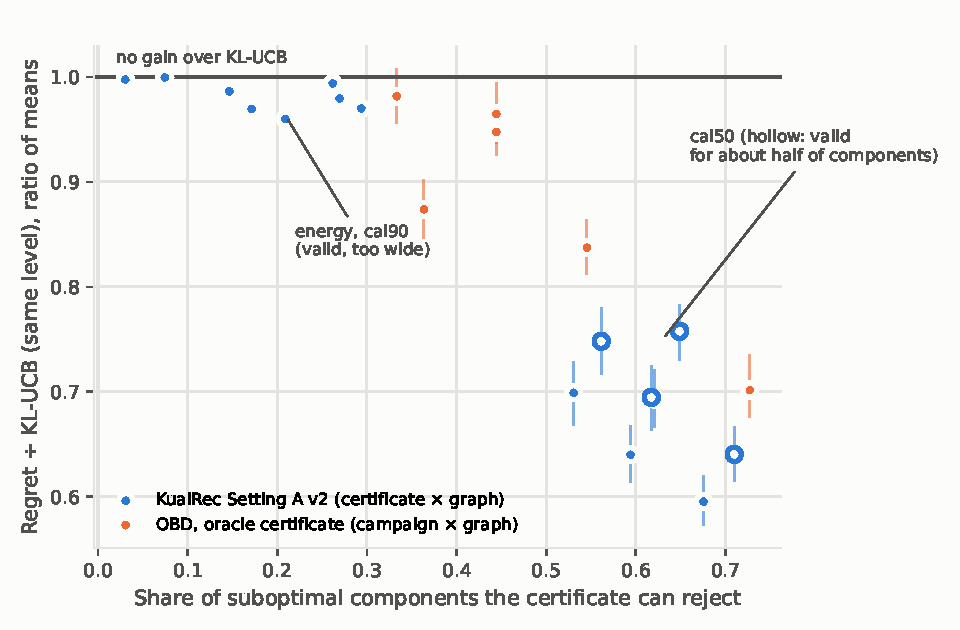
\includegraphics[width=0.95\linewidth]{figures/r1_dose_response.pdf}
\caption{Certified pooling gains with the share of suboptimal components its widths make rejectable: certificate $\times$ graph cells on KuaiRec (360 instances each) and campaign $\times$ grouping cells on the Open Bandit Dataset (20 seeds). Hollow points: widths valid for under 85\% of components. Bars: 95\% bootstrap intervals. A descriptive association, not a per-instance law.}\label{fig:dose}
\end{figure}

\paragraph*{The Open Bandit Dataset} Uniform-random ZOZOTOWN logs~\cite{saito2021obd} (2.69M impressions, three campaigns) give a semi-synthetic fixed-mean test: days 1--3 build attribute or audience groupings and days 4--7 set Bernoulli means (640 trajectories of two million impressions). Oracle audience pooling gains 29.8\% over fixed KL-UCB in the All campaign but 3.5\% in Women, and empirical-Bayes TS has the lowest loss in both. Widths estimated from the prefix cover only 25--70\% of held-out component ranges, so practical certificates remain the open problem.

\paragraph*{Inflation in measured attention} Retrospective panels of 150 Wikipedia articles, fitted on 2022--2023 and evaluated on 2024--2025, show seven-day block-mean inflation $f(7)$ of 5.0--5.3 after weekday adjustment and $f(28)$ of 17.1--17.8: a week of consecutive views carries the information of 1.3--1.9 independent days. Full AR(20) autocovariance predicts these factors more closely than a lag-one shortcut, as Proposition~\ref{prop:cov} suggests.

\paragraph*{Coverage on calibrated worlds} Thirty articles determine six components, stable AR(7) dynamics and correlated Gaussian innovations. Over 730 days and 100 worlds per cell, iid pooling certificates violate an arm or component bound in 56/100 runs for slate size five and 94/100 for size ten (Fig.~\ref{fig:coverage}). Pooling certificates built on the innovation regression, with known or fitted dynamics, show 0/100 violations (Wilson upper limit 3.7\%). Validity is costly: known-model pooling has mean regret 441 against 37.8 for iid confidence at size five, and median terminal width is 0.70 for the ellipsoid of Theorem~\ref{thm:conf} against a best--second gap of 0.135. In a 400-world AR(20) check, known dynamics give 1/100 anytime violations and fitted dynamics 5/100, while replacing AR(20) by AR(1) and dropping cross-arm covariance gives 40/100. Fitted-model coverage is thus measured, not proved; misspecified Cram\'er--Rao and Barankin bounds~\cite{richmond2025mcrb,rosenthal2025barankin} quantify the analogous loss for estimation error, and an all-time analogue for confidence sets is open.

\begin{figure}[t]\centering
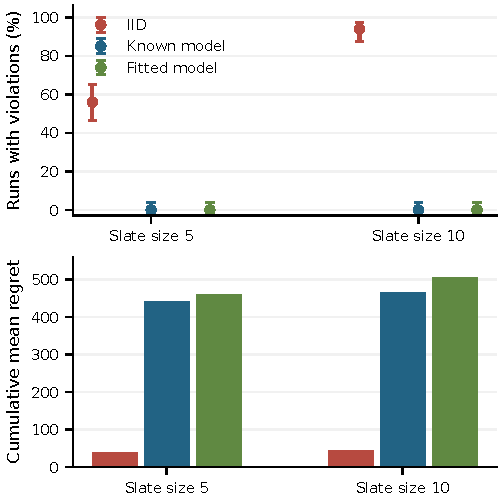
\includegraphics[width=\linewidth]{figures/coverage_cost.pdf}
\caption{Wikipedia-calibrated worlds: coverage and mean-regret cost of pooling certificates, 100 worlds per cell; bars are 95\% Wilson intervals. Correct confidence is far more expensive at this horizon.}\label{fig:coverage}
\end{figure}

\paragraph*{Acting on persistence} On chronological KuaiRec panels (three disjoint 11-day windows, 15 panel--window units, 1,950 trajectories), a joint Kalman filter on long-run means and AR deviations lowers current-oracle loss by 49.3\% [13.4\%, 84.8\%] at budget one and 54.1\% [42.6\%, 67.0\%] at budget five relative to iid Thompson sampling. Its comparison with the last observed value is inconclusive, and graph-shaped shock covariances add little beyond a common factor. Persistence helps decisions; the evidence does not show that a detailed shock graph does.

%=====================================================================
\section{Related work}\label{sec:related}
%=====================================================================

Spectral bandits assume means smooth on a graph~\cite{valko2014spectral,kocak2020spectral}; clustered bandits pool across users or arms~\cite{gentile2014clustering,ban2021local}, tolerate bounded within-cluster deviation at linear regret cost~\cite{wang2023misspecified}, or assume known within-group ranges~\cite{eldowa2026similarities}; Laplacian penalties extend to kernelized rewards~\cite{wu2026laplacian}, and correlated-arm UCB exploits known correlations~\cite{gupta2021correlated}. None checks from data that the structure is valid for the decision. In this venue, graphs have constrained which arm can follow which~\cite{zhang2023graphbandit} rather than related the means, and Thompson-sampling and neural-UCB designs~\cite{zhou2023pts,wang2022neuralbandit} assume independent rewards. Switching bandits forget old data~\cite{garivier2011switching}; AR and latent-state bandits~\cite{chen2023autoregressive,bacchiocchi2024arb,trella2025latent} and Kalman-predicted linear Gaussian systems~\cite{gornet2024restless} model persistence and bound regret against dynamic benchmarks, without confidence for fixed means that survives pooling. Self-normalized bounds~\cite{abbasi2011improved} and confidence sequences~\cite{howard2021confidence} underlie our certificates, and tighter mixtures~\cite{flynn2023martingale} are the route to narrower widths; state-space A/B designs~\cite{shao2026statespace} and sequential tests under Markov dependence~\cite{sethi2026markovian} handle dependence for one test at a time.

%=====================================================================
\section{Conclusion}
%=====================================================================

A graph restriction on means and a graph model for shocks supply different information. The innovation regression yields valid adaptive confidence under known spatiotemporal dynamics, and certified rejection stays sound when it uses that information; confidence built for independence fails under bursty exposure by the factor $f_i(b)$. The data support each mechanism but expose a gap between correctness and usefulness: practical widths are often uninformative, and generic shrinkage or the last observed value captures much of the benefit. A per-contrast confidence sequence that is both valid and narrow is the next problem.

\bibliographystyle{IEEEtran}
\bibliography{references}

\end{document}
